\documentclass[../report/report.tex]{subfiles}
\begin{document}
The VAE provides a probabilistic approach to modeling the data as a distribution around some underlying manifold. This allows us to define a posterior distribution over the latent space, and a distribution over input space which can be used to score inputs, while being able to measure uncertainty over both estimates. Aside from these traditional advantages of a Bayesian approach over traditional methods do we also gain advantages in terms of modeling capabilities?\\
The AE also takes an input vector and maps it to some latent space, however only providing a point estimate on some lower dimensional manifold. AEs are trained by minimizing the reconstruction error of training examples usually measured by mean squared error (MSE), and a weight regularizer:
\begin{equation}
E(\mathbf{x, \theta}) = \lVert \mathbf{x} + \sigma_\theta(\mathbf{x})\rVert^2 + \lambda \ell(\mathbf{\theta}),
\end{equation}
where $\sigma(\cdot)$ represents the application of the autoencoder (encoding followed by decoding) to a particular data example, $\ell(\cdot)$ represents a specific weight decay, and $\lambda$ represents the weight penalty. This can be seen to resemble the variational lower bound:
\begin{equation}
\Func{\mathcal{L}}{\mathbf{\theta}, \phi; \mathbf{x}_i}=\Expect{\Func{q_\phi}{\mathbf{z}_i|\mathbf{x}_i}}{\log \CondFunc{p_\mathbf{\theta}}{\mathbf{x}_i}{\mathbf{z}_i}} - \DivKL{\CondFunc{q_\phi}{\mathbf{z}_i}{\mathbf{x}_i}}{\Func{p_\mathbf{\theta}}{\mathbf{z}_i}},
\end{equation}
in which the first term can be seen as the expected negative reconstruction weight and the second  acts as a regularizer pulling latent variables towards the prior. Rather than defining a distribution in latent variable space, the AE instead provides a point estimate in the bottleneck layer, but the two are analogous in that they provide a lower dimensional representation of an input.\\
Since the latent representation in the VAE is a distribution we have to choose how we use this to create a single decoded example. Both using the mean of the distribution and averaging the output of multiple samples were tried. Using the mean was shown to give an absolute improvement in MSE of about 0.2\%, and so that is the method that is used for further experiments.\\
Instantiations of each model type were trained using the configurations: the encoder and decoder each have one hidden layer of size 500 consisting of, tanh activation functions and using the same $\ell_2$ normalization penalty on the same portion of the MNIST data set. The resulting mean construction errors for the two models for a different size of the latent space/ compression layer are shown in Figure \ref{fig:AE_MSE}.

\begin{figure}[hbt]
\centering
\hspace{0em}
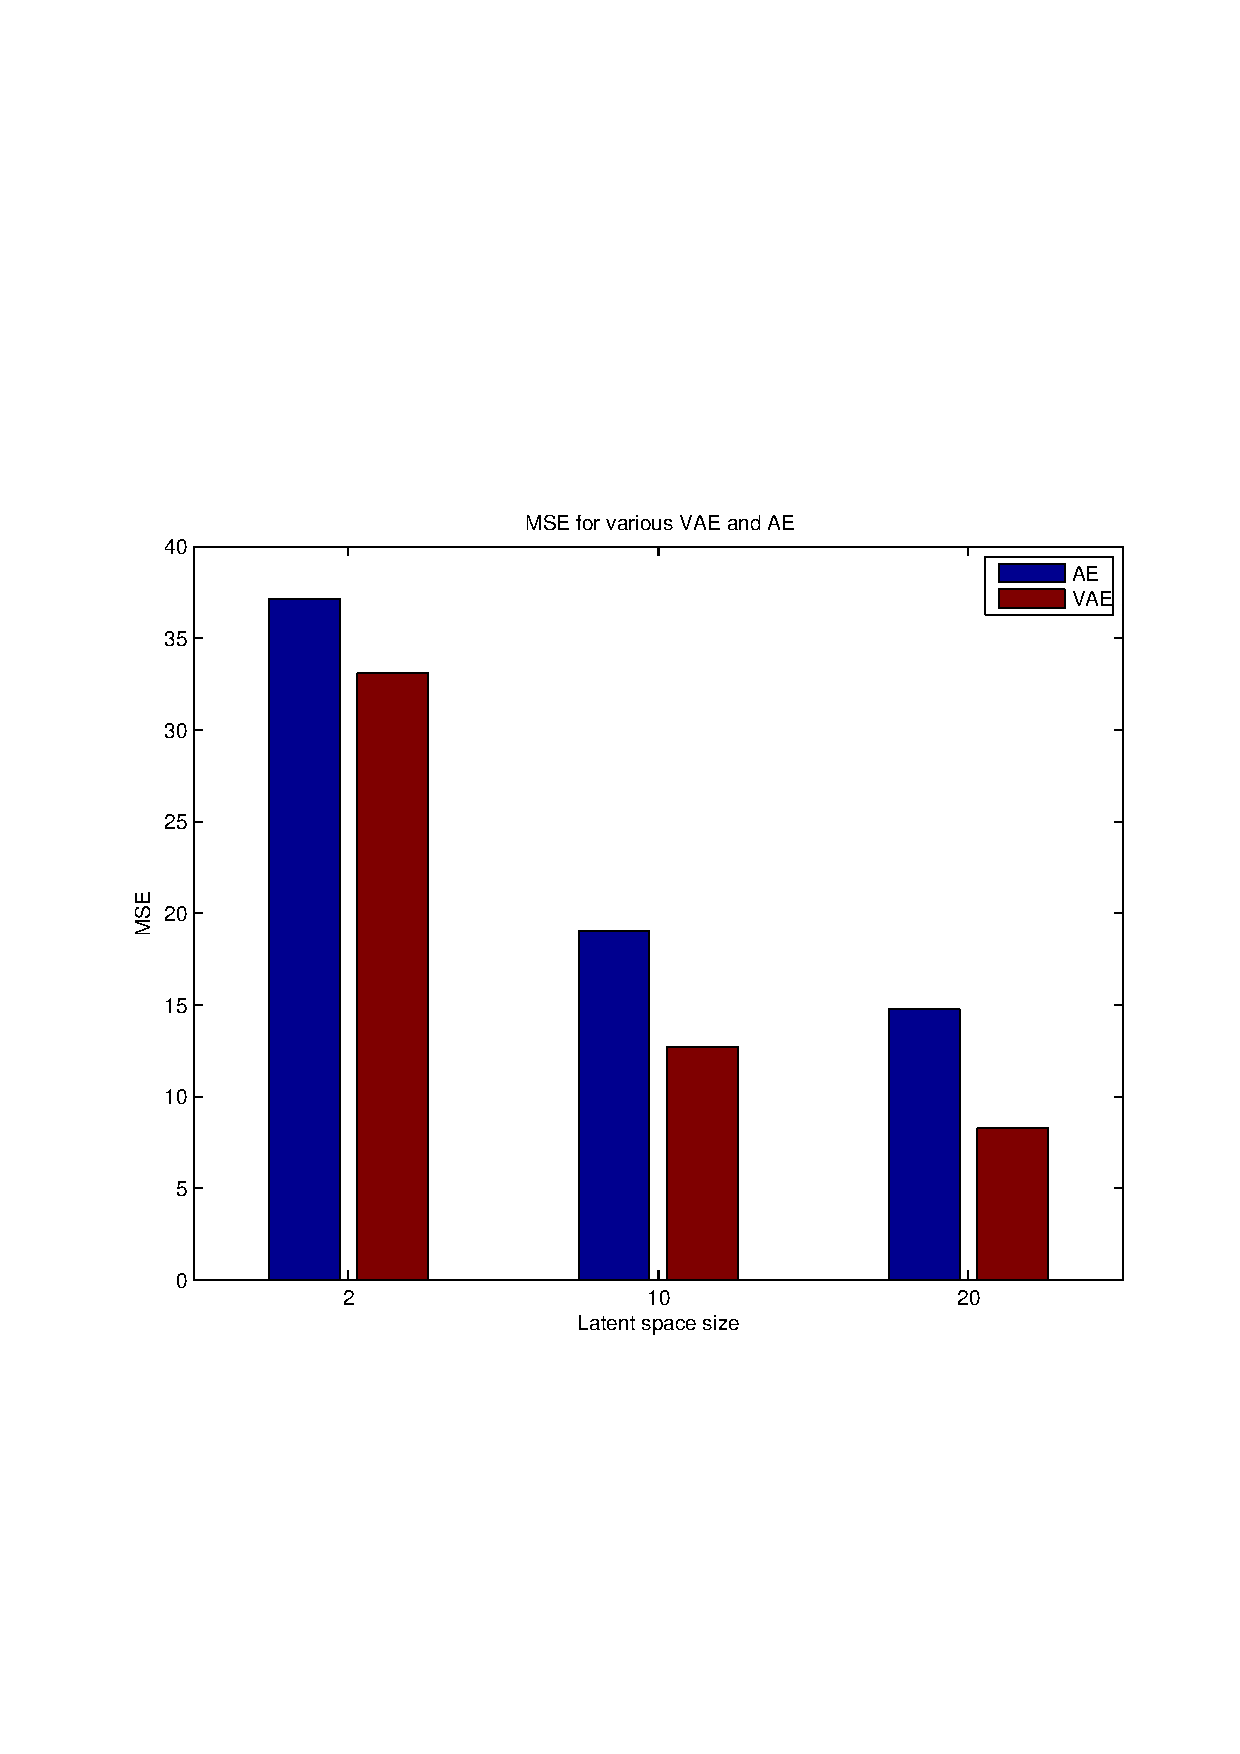
\includegraphics[width=0.4\columnwidth]{../../res/mnist_mse.pdf}
\caption{Comparison of reconstruction error measured by MSE for variational auto-encoder and vanilla auto-encoder for various sizes of representation space}
\label{fig:AE_MSE}
\end{figure}

It can be seen that the variational auto-encoder outperforms the regular auto-encoder for all reduced dimensional sizes. The difference in reconstruction error increases as the size of the latent space/ bottleneck layer increases. This suggests that the difference in performance is due to the better generalization afforded by the variational bayesian approach.\\ Note that the AE is directly trained to minimize the criterion that we have used to compare the two models, whereas VAE is trained to minimize the expected reconstruction rate, which for the discrete case is the binary cross entropy. So despited having an ``unfair advantage'' the auto-encoder still performs worse.\\
To further contrast the two approaches (Figure \ref{fig:AE_recon}) shows specific examples of digits constructed by VAE and AE. It can be seen that generally the VAE produces images that are sharper and more similar to the original digit, with the exception of the number 9 for the 2 dimensional case. It was initially speculated that this would correspond to a higher variance of the posterior, however this was found to not be the case. Looking at the representation of the two dimensional latent space in $?$ we can see that the further right we go the more rightward slanting nines we have, so having a leftward slanting nine would push us away from nines towards the region of weight space containing eights. In such a compressed latent space it seems reasonable to assume that there will be forms of certain digits that are unrepresentable, in this case we have found an unfortunate example on which the VAE performs poorly.\\

\begin{figure}[hbt]
\centering
\hspace{0em}
%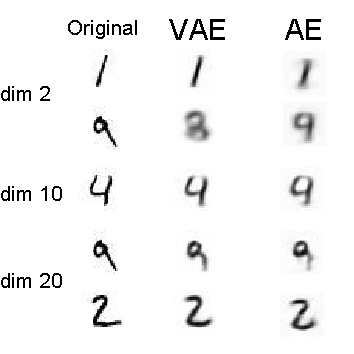
\includegraphics[width=0.4\columnwidth]{../../res/recon_mnist_compre.pdf}
\caption{Examples of the quality of reconstruction of certain digits for VAE and AE}
\label{fig:AE_recon}
\end{figure}

These results must not be taken at face value because, although greatest care was taken to compare the two approaches on an even footing, it is possible that AE is more susceptible to hyperparameter settings, a full investigation of which was not performed here.\\
\end{document}
